\section{Diagramas de estados}
Para especificar os principais processos do projeto foram desenvolvidos diagramas de estados, com o objetivo de demonstrar o processo de criação de um tópico do fórum por parte de um técnico, o processo de aceder e responder a um tópico e o login com ativação de conta, visto que, estas interações são as de maior significância e regradas no \textit{software}.

\subsection{Diagrama de estados criação de tópico}

Com o diagrama de estados de criação de tópico é pretendido demonstrar o processo por parte de um técnico. Assim sendo, primeiramente terá de estar autenticado, caso não esteja, será encaminhado para autenticação. De seguida criará um tópico. Após preencher os campos desejados este poderá confirmar. Caso confirme, é verificado se o tópico possui título. Caso não possua, é determinado como inválido o que levará o técnico a preencher os dados em falta. Contudo, se o título estiver preenchido, é verificado se possui descrição e tipo. Na condição de não possuir descrição ou tipo, é seguido o mesmo fluxo que o caso anterior. Caso contrário é criado um novo tópico. Por fim, na hipótese de o técnico não desejar confirmar o tópico, este poderá cancela-lo, o que o determina como cancelado.

\begin{figure}[htb]
    \centering
    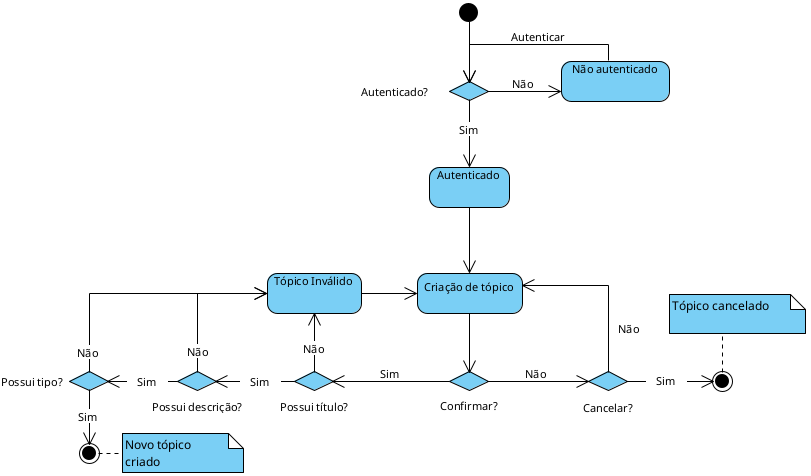
\includegraphics[width=0.9\textwidth]{images/diagramas/estados/criar_topico.png}
    \caption{Diagrama de estados de criar tópico}
    \label{fig:40}
\end{figure}

\newpage

\subsection{Diagrama de estados responder a tópico}

Com o diagrama de estados de responder a tópico é pretendido demonstrar o processo de seleção e de responder a um tópico por parte de um técnico. Assim sendo, primeiramente terá de estar autenticado, caso não esteja, será encaminhado para autenticação. Após a autenticação, o técnico irá por predefinição ver os tópicos em destaque. Nesta listagem selecionará um tópico o que permite responder. Depois da criação do comentário, este poderá confirmar e caso confirme ficará criado, caso contrário ficará cancelado.

\begin{figure}[htb]
    \centering
    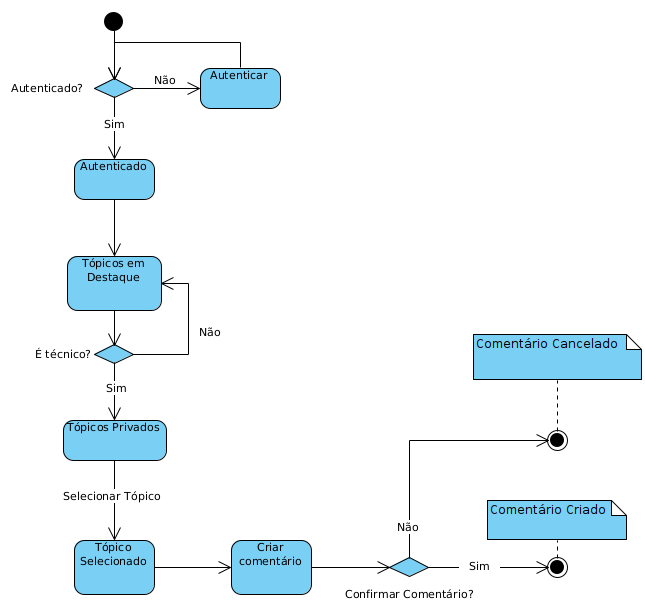
\includegraphics[width=0.7\textwidth]{images/diagramas/estados/responder_topico_tecnico.png}
    \caption{Diagrama de estados de criar tópico}
    \label{fig:41}
\end{figure}

\newpage

\subsection{Diagrama de estados autenticação e validação de conta}

Aquando a realização do login, o técnico indicará as suas credenciais. Todavia, se não estiverem corretas, a autenticação será determinada como incorreta. Caso as credenciais estejam corretas e a conta válida, o técnico ficará automáticamente autenticado. Contudo, na condição de não conter uma conta válida, esta deverá ser validada e para isso, este terá de inserir o código de validação. No caso de o código estar correto, a conta será validada e o técnico ficará autenticado. Caso contrário o código será inválido e este necessitará indicar o código de validação novamente.

\begin{figure}[htb]
    \centering
    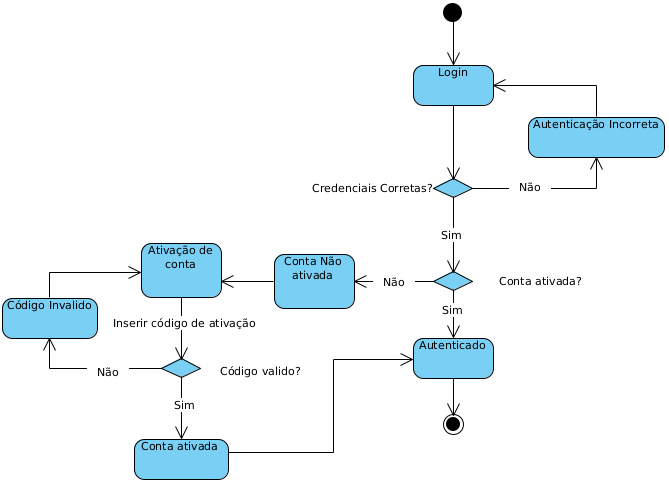
\includegraphics[width=0.7\textwidth]{images/diagramas/estados/autenticacao.png}
    \caption{Diagrama de estados de autenticação e validação de conta}
    \label{fig:42}
\end{figure}